\documentclass[10pt,a4paper]{article}
\usepackage[T1]{fontenc}
\usepackage[utf8]{inputenc}
\usepackage{lmodern}
\usepackage[margin=2.5cm]{geometry}
\usepackage{amsmath,amssymb}
\usepackage{tikz}
\usetikzlibrary{positioning,arrows.meta}
\usepackage{booktabs}
\usepackage{array}
\newcolumntype{L}[1]{>{\raggedright\arraybackslash}p{#1}}
\usepackage{microtype}
\usepackage[hidelinks]{hyperref}
\usepackage{enumitem}
\setlist{itemsep=1pt,topsep=2pt,parsep=1pt}
\setlength{\emergencystretch}{3em}
\newcommand{\lane}{\ell}
\newcommand{\eff}{\mathit{eff}}
\newcommand{\kown}{k_{\mathrm{owner}}}
\newcommand{\kdel}{k_{\mathrm{delegate}}}
\newcommand{\kadm}{k_{\mathrm{admin}}}
\newcommand{\code}[1]{\texttt{\detokenize{#1}}}
\title{\bf The Door Without a Threshold:\\
A Lane-Level Case Study of Configuration Authority\\
in Cross-Chain Bridges}
\author{\large Mingzhao Huang\\[2pt]
\normalsize Shanghai Jiao Tong University\\
\texttt{huangmingzhao@sjtu.edu.cn}}
\date{2026-11-09}
\begin{document}
\maketitle

\begin{abstract}
LayerZero's OApp source-side configuration governs what its endpoint sends, through four doors: the OApp owner, the
endpoint delegate, the EIP-1967 admin, and the send-side verifier set. Security reporting usually compresses
these into a $k$-of-$n$ reading, which presumes that a threshold exists to be read. That presumption fails on
122 of the 730 effective lanes of the arbitrum to dstEid 30101 corridor (132 of the 740 catalogued): there the owner is a role system, a
proxy whose admin exposes no threshold, or an address with no code, so the owner door exposes no $k$: for 62 of them the object exists but exposes none, and for 60
there is no object at all. Reading all four doors lane by lane, with the class assignment read at block 522,563,681 and the capability probe pinned at block
522,662,885 and a named denominator on every count, we find 395 lanes (54.1\%, D2) on which at least one door
can be satisfied by a single key, and the 354 owner-single lanes are held by 225 distinct owners, of which 131 also own weak lanes on base (arbitrum EOA owner set intersected with the base weak-lane owner
set), covering 212 of the 354 lanes (59.9\%). Counting messages instead of lanes reverses the emphasis:
those 395 lanes carry 10.3\% of the 694,619 observed packets, while the 107 undetermined lanes carry 40.2\%,
and the three owner contracts behind 57.0\% of the traffic are two 3-of-5 safes and one role system, none of
them a single key. The lane table, the owner census, the pinned-block probe and the scripts that regenerate
every count are released with the paper, and the procedure is replicated on a second source chain, where 409
of 738 lanes (D2) carry a single-key door. Deployed threshold readings at this granularity do not appear in
the incident and audit literature we compare against, whose full texts contain no threshold call and no
on-chain address; prevalence, harm, and a third chain remain outside the established result.
\end{abstract}

\section{Introduction}
\label{sec:intro}

A LayerZero OApp sends a message when the constraints its own source-side configuration places on it are met. On LayerZero those constraints live in four doors: the OApp owner, the endpoint delegate, the EIP-1967
admin, and the send-side verifier set. Audits enumerate the upgrade path, because an upgrade takes the
system; the doors we read are the ones that change what this source will send without changing code, and
they need no code change and no redeployment. We examine one corridor, arbitrum to dstEid 30101, lane by lane, with the
capability probe pinned at block 522,662,885, and we ask two questions of it.

\paragraph{Two questions.}
\emph{Q1: can every door's constraint be read as a number?} A $k$-of-$n$ reading presumes that a threshold
exists. We test that presumption per lane rather than per protocol, and we keep three outcomes apart: a
threshold that is returned, an object that exists but exposes none, and no object at all. \emph{Q2: does the
number correspond to the traffic the door guards?} A share of lanes answers a question about the catalogue;
an operator acts on a question about messages. We count both and report where they diverge.

\paragraph{What we find.}
On the 730 effective lanes of the corridor, 395 (54.1\%, D2) have at least one door a single key can satisfy.
On 122 of the 730 lanes (132 of the 740 catalogued) the owner door exposes no $k$ at all, and the six classes we sort them into share no fix: a renounced
owner is a door nobody can open, a role system is a door whose constraint is a predicate rather than a
count, and a phantom entry is not a lane. Counted in messages the emphasis reverses: the single-key lanes
carry 10.3\% of the 694,619 packets, and the undetermined lanes carry 40.2\%. The three owner contracts that
carry 57.0\% of the traffic are two 3-of-5 safes and one role system; none of them is a single key, and the
largest is the one whose threshold cannot be read.

\paragraph{Contributions.}
\begin{enumerate}[leftmargin=1.2em,itemsep=2pt,topsep=2pt]
\item A per-lane reading of four configuration doors on 730 effective lanes, with a named denominator for
every count and a three-state decision that separates an absent object from an unreadable one.
\item A count, and a partition, of the 122 lanes on which a $k$-of-$n$ metric has nothing to read. The
partition is the result rather than a qualification: it is why a share-only report cannot state this
finding, and it survives as a partition on a second source chain.
\item A message-weighted reading of the same lanes. The lane ordering and the traffic ordering disagree
(10.3\% against 40.2\%), which changes which door an operator should look at first.
\end{enumerate}

\paragraph{Scope of the evidence.}
The lane table, the owner census, and the capability probe at the pinned block are released with the
scripts that regenerate every count, and a reader can re-derive each number from them. The evidence supports
statements about this corridor at that block; it does not measure prevalence outside the catalogue, it does
not price what sits behind a door, and it does not test a third source chain. Those three remain outside the
established result, and Section~\ref{sec:threats} states them as conditions that would overturn it rather
than as caveats.

\section{Model: four doors, one minimum, three states}
\label{sec:model}

\subsection{Four doors and one minimum}
A lane is as weak as the minimum over its four doors. For a lane $\lane$ we read the OApp owner's
threshold $\kown$, the endpoint delegate's threshold $\kdel$, the EIP-1967 proxy admin's threshold
$\kadm$, and the effectiveness $\eff$ of the send-side verification set, the number of independent
domains a message must satisfy; the attack surface we report is
\begin{equation}
\mathrm{attack}(\lane)=\min\bigl(\eff(\lane),\kown(\lane),\kdel(\lane),\kadm(\lane)\bigr),
\end{equation}
so a lane is single-key when that minimum is one, and the complementary minimum over the three
authority doors alone separates a weak authority from a weak verifier set.

\subsection{Three states}
Every door is in exactly one of three states, and the paper's third result depends on keeping them
apart: \emph{threshold}, when a $k$ is present and readable; \emph{unreadable}, when the object exists
but exposes no threshold, as with a role table or an unresolved proxy admin; \emph{absent}, when there
is no object to read, as with a renounced owner or an address with no code. A two-state reader must
record the last two as unknown, which converts a fact about the protocol into a fact about our access;
the 122 lanes of Section~\ref{sec:notmeasurable} exist because of that difference.

\subsection{Why a single-key door is weak}
Three mechanisms make a door with $k=1$ weaker than its code suggests, and they are why we report the
minimum rather than an audit finding.

The first is quorum collapse. A threshold of $k$ is a statement about how many independent compromises an
attacker needs; $k=1$ reduces that number to one, so the strength of the door equals the strength of a single
key, whatever the contract around it looks like. The second is that the door needs no code change. An
upgrade takes a deployment, and a deployment is slow enough that a defender can notice; a configuration
change needs only a transaction and takes effect on the next message. The third is that the change does not have to break a
check. The delegate is the address that configures the OApp's libraries, so a key that can replace the
delegate reaches the setting that decides who may attest, and an attacker who gets there does not forge a
message at all: he changes the set of parties whose word counts.

None of this is measured harm. We read structure, and structure is what these three mechanisms act on: the
395 lanes below are weak in the sense that one compromise is enough, not in the sense that one happened.
\subsection{Denominators, named before any number is read}
Every count carries one of five labels, because the two chains do not share a catalogue: D1 = 740
catalogued lanes on arbitrum, including phantom entries; D2 = 730
effective lanes on arbitrum, 738 on base, after removing entries with no code and no packets; D3 = 639
lanes with a readable record for at least one door; D4 = 608 lanes whose owner door is readable on
arbitrum, 610 on base \code{[CLAIMS:A0]}. The base catalogue is a different set: D1b = 754 catalogued lanes, so
base's removal count divides by D1b, not by D1 \code{[BASE-LANES:3]}. A share of 730 and a share of 608 answer different questions,
and no number below appears without its label.

\begin{figure}[t]
\centering
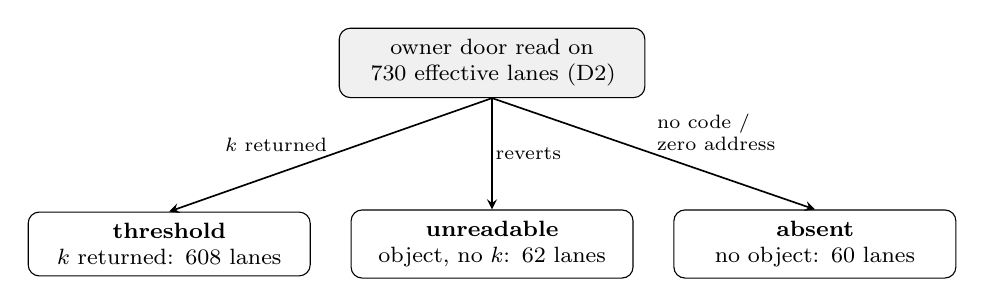
\begin{tikzpicture}[
  every node/.style={font=\footnotesize},
  box/.style={draw, rounded corners, align=center, inner sep=4pt, text width=3.3cm},
  rootbox/.style={box, fill=black!6, text width=3.6cm},
  leaf/.style={box},
  arr/.style={->, >=stealth, semithick}]
\node[rootbox] (root) at (0,0) {owner door read on\\730 effective lanes (D2)};
\node[leaf] (thr) at (-4.1,-2.3) {\textbf{threshold}\\$k$ returned: 608 lanes};
\node[leaf] (unr) at (0,-2.3)   {\textbf{unreadable}\\object, no $k$: 62 lanes};
\node[leaf] (abs) at (4.1,-2.3) {\textbf{absent}\\no object: 60 lanes};
\draw[arr] (root.south) -- node[above left, align=right, font=\scriptsize, fill=white, inner sep=1pt] {$k$ returned} (thr.north);
\draw[arr] (root.south) -- node[right, font=\scriptsize, fill=white, inner sep=1pt] {reverts} (unr.north);
\draw[arr] (root.south) -- node[above right, align=left, font=\scriptsize, fill=white, inner sep=1pt] {no code /\\zero address} (abs.north);
\end{tikzpicture}
\caption{The three-state decision on the owner door, with the lane counts the partition produces. Only the
leftmost branch yields a $k$; a two-state reader must file the other 122 lanes either as one key or as
ignorance, and both readings are wrong for different reasons.}
\label{fig:states}
\end{figure}
\section{Measurement: the distribution on 730 lanes}
\label{sec:measurement}

\paragraph{The corridor.}
The corridor holds 730 effective lanes at one destination, dstEid 30101 (D2), and the reading is
at lane granularity, not at application granularity: an application can hold several lanes, and Table~\ref{tab:twochains}
says which population each column divides by. We use one destination because it is the only one at
which every lane's send-side configuration can be paired with the receiving endpoint's view at a
recorded block.

\begin{table}[t]
\centering
\small
\caption{Two source chains read at one destination. Counts are lanes unless the row says owners; the
label after each count is its denominator. Source: \code{[RESULTS:R1,R2,R3,R7]} for arbitrum and
\code{[BASE-LANES:3]} for base.}
\label{tab:twochains}
\begin{tabular}{@{}lrr@{}}
\toprule
quantity & arbitrum & base\\
\midrule
effective lanes & 730 (D2) & 738 (D2)\\
at least one single-key door & 395 (D2) & 409 (D2)\\
share of effective lanes & 54.1\% (D2) & 55.4\% (D2)\\
undetermined & 107 (D2) & 105 (D2)\\
owner door single-key, all readable lanes & 354/608 (D4) & 358/610 (D4)\\
share of readable owner lanes & 58.2\% (D4) & 58.7\% (D4)\\
owner door single-key, inside the weak lanes & 354/395 (D2) & 358/409 (D2)\\
share of single-key-door lanes & 89.6\% (354/395) & 87.5\% (358/409)\\
distinct single-key owners & 225 (D4) & 255 (D4)\\
phantom lanes removed & 10 (D1) & 16 (D1b)\\
pessimistic end of the share & 67.9\% (D2) & ---\\
\bottomrule
\end{tabular}
\end{table}

\paragraph{One share, one interval.}
The single-key share is 54.1\% (D2) of 730 lanes, and Table~\ref{tab:twochains} gives its pessimistic end,
reached by treating every undetermined lane as single-key \code{[RESULTS:R2]}. We report the point and the
end together: the width between them is a statement about how many lanes our access leaves open, and
summing the two into one coverage figure would hide exactly that.

\paragraph{Lanes are not traffic.}
A share of lanes is not a share of activity. Of the 740 catalogued lanes only 184 sent a packet in the
twelve months we observe, and the 694,619 packets that come from catalogue lanes split very differently
from the lane counts: 395 single-key lanes (54.1\%, D2) carry 71,669 packets (10.3\%), 228 lanes that need
two keys everywhere carry 343,672 (49.5\%), and the 107 undetermined lanes carry 279,278 (40.2\%). The
door we cannot read is the door in front of the traffic; the door we can read as single-key is in front of
little of it. We report both counts for that reason, and we do not treat either as the headline.
\begin{table}[t]
\centering
\small
\caption{The same partition counted two ways. Lane counts divide by 730 (D2); packet counts divide by the
694,619 packets that come from catalogue lanes. Source: \code{[TRAFFIC-MIX]}, \code{[KEY-TRAFFIC:4]}.}
\label{tab:traffic}
\begin{tabular}{@{}lrrrr@{}}
\toprule
class & lanes (D2) & share of lanes & packets & share of packets\\
\midrule
at least one single-key door & 395 & 54.1\% & 71,669 & 10.3\%\\
two or more keys everywhere & 228 & 31.2\% & 343,672 & 49.5\%\\
undetermined & 107 & 14.7\% & 279,278 & 40.2\%\\
\midrule
total & 730 & 100\% & 694,619 & 100\%\\
\bottomrule
\end{tabular}
\end{table}

\paragraph{A lane read end to end.}
Take \code{0x19cfce47ed54a88614648dc3f19a5980097007dd}, one of the three lanes behind the largest owner in
the traffic table. The send-side configuration reports an effective verifier count of 3, so $\eff=3$ \code{[lane-doors]}. \code{owner()} returns \code{0x184257d5b9e25a12d1dcafb697bfaafe0f5ca150}, which has
7,197 bytes of code and answers \code{getThreshold()} with a revert, so the owner door is \emph{unreadable},
not \emph{absent} and not a threshold. The delegate and admin doors expose nothing on this lane. The minimum
is therefore undetermined: no readable door pins it to one, and the door that would pin it cannot be read.
Classified by what the chain exposes, the lane is a role system. It is one of the 122, it is one of the three lanes behind
the owner that carries 22.8\% of the corridor's packets, and it contributes nothing to a single-key share. a share-only
instrument reports it either as single-key or as missing, and the released procedure reports what it did:
queried, answered, no object.
\paragraph{The destination side.}
The four doors above are read on the source chain. We also resolved the destination object for each lane:
the source OApp's \code{peers(30101)} names the receiving contract, and the same three-state rule applies to
its owner. The lookup succeeds for 181 of the 730 lanes. The other 549 are not unreadable in the sense of
Section~\ref{sec:notmeasurable}, because the chain gives three different answers. Fifty-nine return an
explicit zero address, so the corridor has no peer recorded there at this block; 478 return nothing at all,
140 of which report a revert (138 with no reason string, one PB-NFUN-01, one an ownership revert); and 12
return an empty word. We report the three counts separately and classify none of them as a door. Of the 181,
two lanes have a destination owner that one key can satisfy (269 of the 694,619 packets), 79 expose no
threshold, and 100 require two keys or more.

The asymmetry is the result, and it holds on one denominator. Among those same 181 lanes the source-side
minimum is one on 74 of them (40.9\%), while the destination owner is single-key on two; the multisig
majority sits on the receiving side. Lanes the lookup could not resolve are not counted on either side, and
we do not impute a state to them.
\paragraph{The second chain, structurally.}
Base does not merely reproduce the totals. Among the lanes that are weak on it, the owner door is single on
87.5\% (358 of 409) against 89.6\% on arbitrum (354 of 395): the door at which the weakness sits is the same
on both chains. What differs is how many of the four doors are at one. On base 48.9\% of the weak lanes have at
least two of the four doors open to a single key (200 of 409), against 33.7\% on arbitrum (133 of 395), so base has more rooms with two doors at one. We record thresholds, not addresses, so we cannot tell whether the two doors at one are opened by the same key, and we do not claim that they are. A single share would have hidden this; the partition shows
it, because it keeps the doors apart.
\paragraph{The second chain.}
Base reproduces the partition at 409 of 738 effective lanes (D2), with 358 of those lanes owner-single-key
against 354 on arbitrum (D4) \code{[BASE-LANES:3]}. The replication is not an independence claim: the two chains
share owners, as Table~\ref{tab:bounds} records, so the columns overlap and we do not add them.

\paragraph{Where the single key sits.}
The 354 owner-single-key lanes (D4) rest on fewer accounts than lanes; resolving those accounts shows
that 131 of the 225 owner addresses also own weak lanes on base, covering 212 of the 354 lanes
\code{[RESULTS:R8,R9]}. That concentration is the only place in this paper where key reuse is measured;
elsewhere the unit is the lane.

\section{Related work}
\label{sec:related}

The literature that comes closest to this paper falls into four groups, and the gap we address is visible
from the way each group chooses its unit of analysis.

\subsection{Incident and vulnerability studies}
Samiha et al.~\cite{samiha2026attack} assemble 48 evidence-supported incidents between January 2022 and
August 2026 and organise them into six trust-violation patterns, of which credential seizure is one. Wang
et al.~\cite{wang2026cvv} take verification defects as their object and draw their sample from audit reports.
Hedge Funds on a Swamp~\cite{hedgefunds2025} builds a layered threat model over thirteen bridges, twenty-three
attack vectors and forty-three scenarios. All three start from an event: something failed, and the
classification explains how. None of them reports what the configuration of an unbroken deployment looks
like, and neither reports a deployed threshold reading, and their full texts contain no on-chain address, so a reader cannot join their
incidents to a lane.\footnote{Wang et al.~\cite{wang2026cvv} report 588 samples in their sample section and
209 audit reports over 27 projects in their dataset table; we cite the table figures and do not reconcile
the two.} Our verdict: their unit is the event, so the configuration of an unbroken deployment is outside their frame.

\subsection{Measurements of interoperability}
A second strand measures the deployed ecosystem rather than its failures. The Price of
Interoperability~\cite{priceinterop2026} observes twenty chains and sixteen bridges over 2022--2025 and
treats the multi-chain ecosystem as a temporal hypergraph, which lets it speak about structural redundancy.
XSplicer~\cite{xsplicer2026} reconstructs cross-chain transactions across 131 bridges and reports that only
16.79\% of them offer complete public traceability. Interoperability Effects~\cite{interop2026} uses panel
regressions to relate interoperability to TVL and revenue. These papers share our interest in the deployed
state, and they measure liquidity, connectivity or economic outcome; none reads the authority that decides
what a source sends, which is the quantity a single compromised key acts on. Our verdict: the deployed state is measured, but not the authority in it.

\subsection{Detection and audit tooling}
A third strand builds instruments. BridgeShield~\cite{bridgeshield2025} reconstructs behaviour graphs from
execution traces and detects attacks on them; GoAT-X~\cite{goatx2026} organises LLM-assisted auditing around
a reasoning graph; COBALT-TLA~\cite{cobalttla2026} synthesises TLA+ specifications and model-checks them,
reproducing the Nomad failure; IntentFuzz~\cite{intentfuzz2026} fuzzes intent-based bridges. These tools
consume a model, and a model carries trust assumptions. Our contribution is orthogonal: we read the
assumptions a deployment actually ships, per lane, so that a model can be instantiated with what is there
rather than with what the protocol documentation says should be there. Our verdict: these tools are complementary rather than competing. They consume the assumptions we read.

\subsection{Taxonomies, practice, and quorum theory}
Zamyatin et al.~\cite{zamyatin2021sok} taxonomise cross-chain communication and its trust assumptions;
Bitcoin bridge taxonomy~\cite{bitcointaxonomy2025} does the same for one asset class; Alfaro et
al.~\cite{alfaro2025comparative} compare four bridge archetypes on a table of metrics whose values the
authors label illustrative. Practice fixes the unit at the bridge as well: the L2BEAT risk
framework~\cite{l2beat2024risk} grades bridges on dimensions assessed from documentation and interviews,
which is the right granularity for a dashboard and the wrong one for a lane. Quorum theory supplies the
assumption our 122 lanes break: Malkhi and Reiter~\cite{malkhi1998quorum} define a quorum system over a set
of servers and ask which intersection properties hold, and the object being read is a threshold. On 122 of
the 730 lanes there is no such object, so theory does not apply as stated. Not because the deployment
is unsafe, but because the metric presupposes a $k$ the chain does not expose.

\subsection{What none of them reports}
Across the four groups the unit is the incident, the ecosystem, the tool's input model, or the bridge.
None of them reports, for a set of lanes with a denominator, how many keys a change requires at each door,
and none of them separates a door that is unreadable from a door that does not exist. That separation is
what makes a share-only report unable to state the finding this paper reports.

\section{Why it is not all measurable}
\label{sec:notmeasurable}

\paragraph{The 132 lanes.}
On 122 of the 730 lanes the owner door is not threshold-expressible (132 of 740 catalogue them, the other ten being the phantom entries), and all 122 return a definite answer when
queried (D2): the answer is that the object a threshold would describe does not exist \code{[RESULTS:R5]}.
We sort them into six classes by what the chain exposes, and Table~\ref{tab:classes} reports, for each
class, whether a $k$ can be produced from chain state alone. For none of the 122 can it; 15 of them are nevertheless decided by a different door being one, which is what leaves the 107.

\begin{table}[t]
\centering
\small
\caption{The 132 lanes with no readable owner door (D1), by what the chain exposes; in D2 the same rows are 56, 54, 6, 5, 1, 0 and total 122.
Source: \code{[RESULTS:R5]}, \code{[OWNER-DOOR-CLASSES:2]}.}
\label{tab:classes}
\begin{tabular}{@{}L{4.2cm}r L{4.4cm} L{4.1cm}@{}}
\toprule
class & lanes (D1) & what the chain exposes & $k$ from chain state\\
\midrule
role system, no threshold & 56 & contract without \code{getThreshold()} & no: role enumeration\\
proxy admin unresolved & 5 & proxy whose admin has no threshold & no: second recursion\\
proxy, no admin slot & 1 & proxy with no admin slot & no: implementation table\\
renounced owner & 6 & \code{owner()} is the zero address & n/a: the door is closed\\
no owner, no implementation & 54 & \code{owner()} reverts or is empty & no: custom authority\\
no code on either chain & 10 (D1 only) & no code, never sent a packet & n/a: not a contract here\\
\bottomrule
\end{tabular}
\end{table}

\paragraph{Why the partition is the result.}
The six classes do not share a fix, which is why one count cannot stand for them: a renounced owner is
a door that no one can open, so counting those 6 lanes as undetermined understates the deployment; a
role system is a door that exists with a threshold that is a predicate over roles, so a single $k$ is the
wrong object; a phantom entry has no code on either chain, so leaving those 10 lanes in the denominator
dilutes every share in the paper.

\paragraph{Fifteen boundaries, stated as limits on what the numbers can mean.}
Table~\ref{tab:bounds} lists them; the two that move the most are the catalogue and the destination.
The catalogue's recall is unmeasured, so a lane we never saw can neither raise nor lower any count. And
every lane is read at one destination, which fixes the verifier set and leaves the authority doors
untouched. Neither boundary can be closed by reading more lanes of the same kind.

\begin{table}[t]
\centering
\small
\caption{Boundaries that bound every count in this paper. Source per row; no row is a defect of the
measurement, each is a limit of its scope.}
\label{tab:bounds}
\renewcommand{\arraystretch}{1.08}
\begin{tabular}{@{}L{5.6cm}L{9.3cm}@{}}
\toprule
boundary & what it limits\\
\midrule
catalogue recall unmeasured (D1) & shares are shares of the catalogue, not of all deployed lanes; no recall figure is claimed \code{[CLAIMS:8]}\\
one destination, 30101 (D2) & verifier sets are fixed by the destination; a second one is untested here. All four doors are read on the source chain: the receiving OApp's own owner and receive configuration at 30101 are not read\\
two source chains & a replication of a procedure, not a sample of bridges \code{[BASE-LANES:3]}\\
overlapping owner sets (D4) & 133 owners appear on both chains, so the columns are not independent\\
undetermined lanes & 107 lanes remain open (D2); the interval carries the uncertainty, not a share\\
phantom entries & 10 catalogued addresses have no code on either chain (D1)\\
exposure, not harm & no value is priced behind any door, so no loss is claimed \code{[RESULTS:R6]}\\
block-time snapshot & a door can change after the recorded block; the reading is a state, not a trend\\
lanes are not traffic & only 184 of 740 catalogued lanes sent a packet in the window; a lane share is not an activity share \code{[KEY-TRAFFIC:4]}\\
sender to owner mapping & 25,509 of 720,128 packets (3.5\%) come from senders absent from the owner census, and are unmapped\\
role systems are not enumerated & a role-governed owner is reported unreadable, not resolved to its role holders\\
multisig sets rotate & a Safe's $k$ of $n$ is read at one block; signer sets can change afterwards\\
third-chain phantoms & phantom detection tests code on two chains; an address with code only on a third would be misfiled\\
capability is not exploitability & a single-key door is authority, not a demonstrated attack path\\
classes describe what the chain exposes & the six classes partition observable state, not the intent of the deployer\\
\bottomrule
\end{tabular}
\end{table}

\section{Limitations and reproducibility}
\label{sec:threats}

\subsection{Limits of the evidence}
The lane table is a catalogue, and its recall of the deployed population cannot be measured under
D1, so every share is a share of what the catalogue contains: a lane we never saw can neither raise nor
lower any count. All lanes are read at one destination, which fixes the verifier set and leaves the
authority doors untouched, and at one block, so a door that changed afterwards is not in the reading. The
two source chains share owners (133 addresses appear on both), so their columns are a replication of a
procedure rather than independent samples, and we do not add them. The 107 undetermined lanes remain in the
denominator, and the interval, not a share, carries what they could change: treating every undetermined lane whose door is open as single-key moves the corridor to 67.9\% (D2); the six
renounced owners are closed doors, not unknowns, and are excluded from that bound.

These are demonstrations within a tested environment. Prevalence outside the catalogue, deployment
reachability of any particular key, attack rates, and the value sitting behind any door remain outside the
evidence: we price nothing, so no loss is claimed, and a single-key door is a capability rather than a
demonstrated attack path. What would overturn the partition is stated as three queryable conditions: a
phantom address acquiring code on a third chain, a \code{getThreshold()} becoming reachable through a
second-level proxy, or a single-key owner turning out to be a contract wallet with an internal threshold of
two or more. Each is a check a reader can run against the released procedure rather than a caveat.

\subsection{Evidence provenance and disclosure}
Every observation is of public chain state at a recorded block; no private key, node, or off-chain record
was used. We identify configurations rather than vulnerabilities: the released table ranks lanes by packets and
by threshold, not by ease of exploitation, and it was not sent to any protocol team before release. The raw reads are regenerable from the pinned block, and the
only derived file in the artifact is the packet aggregation, whose source hash is recorded so that the
derivation can be repeated. Where we quote a number from another paper we quote its table rather than its
abstract, and we say so in the footnote when the two disagree.

\subsection{Artifact availability}
The artifact is released at \url{https://github.com/HMZ-fig/door-without-threshold} and re-derives the lane-level counts without network access:
\code{python3 code/reproduce.py} runs twenty-eight assertions: 740 and 730 lanes, 395 at least one
single-key door, 228 at two or more keys everywhere, 122 lanes with no readable owner door (107 of them
undetermined), the six classes over those 122, the
message shares 10.3/49.5/40.2\%, and the base column at 409 of 738 with 358 owner-single. It exits non-zero if any of them drifts. Two further
checks run beside it: one re-derives every number the text quotes and fails on any that drifts, and
one asserts a runnable condition for each row of Table~\ref{tab:bounds}. The directory holds the lane table, the six-class assignment, the owner
census, the per-OApp packet counts and the second chain's table, each listed with its SHA-256 in the
artifact's README, together with the scripts and a statement of what is not released.

\subsection{Remaining questions}
Three questions follow directly and none is answered here. Does the partition hold on a third source
chain, or is the absence of a threshold a property of the two deployments we read? Can a role-governed
owner be resolved to its role holders well enough to replace a $k$ with something comparable, and would
that change the traffic ordering? And what sits behind the doors, the value a key could redirect,
which needs price data we do not have and did not use.

\section{Conclusion}

\paragraph{What the number is.}
On the 730 effective lanes of one corridor, 395 have at least one door a single key can satisfy, and the owner-single lanes are held by 225 distinct addresses, 131 of which also own weak lanes on base. Counted in
messages the emphasis reverses: those 395 lanes carry 10.3\% of the 694,619 packets we observe, while the
107 lanes whose minimum we could not decide carry 40.2\%. The door we can read as single-key is in front of
little of the traffic; the door we cannot read is in front of most of it.

\paragraph{What it is not.}
It is not a harm estimate, and it is not a claim about bridges in general. No value is priced behind any
door, both chains are read at one destination, and the catalogue's recall is unmeasured, so every share is a
share of what we could see. What would overturn the partition is stated as
three queryable conditions rather than as a caveat.

\paragraph{What a reader can take.}
Three things. A three-state rule that classifies an owner door as threshold, unreadable, or absent, and
refuses to file the last two together; a count, on 122 lanes, of the cases where a $k$-of-$n$ metric has no
object to read, which is why a share-only report cannot state this finding; and a released procedure that
reproduces the partition on a second source chain if the first one was an artefact.
\section*{AI contribution disclosure}

\textbf{Substantial AI contribution.} AI systems contributed to source analysis, proof development,
experimental execution and verification, and manuscript preparation and revision. The author remains
responsible for understanding, verifying, and defending the claims, evidence, citations, and code, and for
the integrity of the submitted work.
\begin{thebibliography}{9}
\bibitem{samiha2026attack} I. Samiha, Y. Rahman, R. Mukta. \emph{Attack Patterns in Cross-chain Bridges: A Trust-based Empirical
Analysis}. arXiv:2611.01587, 2026.
\bibitem{wang2026cvv} Y. Wang, Y. Guo, J. Chen, H. Zhang, Y. Sun. \emph{Understanding Verification Vulnerabilities
in Cross-chain Bridges: An Empirical Study}. arXiv:2610.13170, 2026.
\bibitem{hedgefunds2025} \emph{Hedge Funds on a Swamp: A Layered Threat Model for Cross-Chain Bridges}.
arXiv:2507.06156, 2025.
\bibitem{priceinterop2026} \emph{The Price of Interoperability}. arXiv:2604.03083, 2026.
\bibitem{xsplicer2026} \emph{Bridging the Opacity: Cross-Chain Transaction Reconstruction (XSplicer)}.
arXiv:2609.18158, 2026.
\bibitem{interop2026} \emph{Interoperability Effects}. arXiv:2605.12508, 2026.
\bibitem{bridgeshield2025} \emph{BridgeShield: Behaviour-Graph Detection for Cross-Chain Bridges}.
arXiv:2508.20517, 2025.
\bibitem{goatx2026} \emph{GoAT-X: Audit Reasoning Graphs for Cross-Chain Contracts}. arXiv:2604.24341, 2026.
\bibitem{cobalttla2026} \emph{COBALT-TLA: Specification Synthesis and Model Checking for Cross-Chain
Protocols}. arXiv:2604.12172, 2026.
\bibitem{intentfuzz2026} \emph{IntentFuzz: Protocol-Aware Fuzzing for Intent-Based Bridges}. arXiv:2609.13004,
2026.
\bibitem{bitcointaxonomy2025} \emph{Bitcoin Cross-Chain Bridge: A Taxonomy}. arXiv:2509.10413, 2025.
\bibitem{zamyatin2021sok} A. Zamyatin et al. \emph{SoK: Communication Across Distributed Ledgers}. In
Financial Cryptography and Data Security (FC), 2021. doi:10.1007/978-3-662-64331-0\_1.
\bibitem{alfaro2025comparative} Alfaro, Calderon, Espinoza. \emph{Comparative Security Analysis of Cross-Chain
Protocols: An Empirical and Metrics-Based Approach}. IEEE CONCAPAN XLIII, 2025. doi:10.1109/CONCAPAN66820.2025.11512555.
\bibitem{l2beat2024risk} L2BEAT. \emph{L2Bridge Risk Framework}. 2024. \url{https://forum.l2beat.com/t/l2bridge-risk-framework/31}.
\bibitem{malkhi1998quorum} D. Malkhi, M. Reiter. \emph{Byzantine Quorum Systems}. Distributed Computing, 1998.
doi:10.1007/s004460050050.
\end{thebibliography}

\appendix

\section{Reproducibility protocol}
\label{app:protocol}

\paragraph{What a reader runs.}
The artifact is a directory with four data tables and two scripts, and one command reproduces every number
in this paper without network access:

\begin{quote}\ttfamily
python3 code/reproduce.py\quad\# 14 checks, exit 0 when the paper's numbers hold
\end{quote}

\begin{sloppypar}
The script loads \code{lane-doors.csv}, \code{owner-door-classes.json}, \code{owner-census.csv},
\code{packets-per-oapp.csv} and the second chain's table, and asserts each quantity the text quotes: 740 and
730 lanes, 395 at least one single-key door, 228 at two or more keys everywhere, 107 undetermined, the six
classes summing to 107, the message shares 10.3/49.5/40.2\%, and the base column at 409 of 738 with 358
owner-single. Each file is listed with its SHA-256 in the artifact's README, so a reader can confirm the
inputs before trusting the output.
\end{sloppypar}

\paragraph{What is released, and what is not.}
Released: the lane table (one row per corridor lane, four doors and the minimum), the six-class assignment
for the 132 lanes of D1 (122 in D2), the OApp to owner census, the per-OApp packet counts, and the second chain's table.
Not released: the raw RPC responses, which are regenerable from the pinned block, and the 42\,MB packet
corpus, whose aggregation script and SHA-256 are given so the derivation can be repeated. The packet
aggregation is the only derived file in the artifact; everything else is a direct read.
\paragraph{How to read the bracketed tags.}
A tag such as \code{[RESULTS:R2]} or \code{[BASE-LANES:3]} names a row in the ledger released with this
paper, not an external citation. The ledger is generated by the same scripts that produce the tables here,
so a tag is a provenance pointer: it says which released row a number comes from, and a reader who runs the
scripts can check that the row and the number still agree. No claim in this paper depends on material that
is not released alongside it.
\paragraph{The decision rule, written so it can be coded.}
A lane's owner door is read in three steps. First, if the OApp address has no code on this chain and has
never sent a packet, the lane is a phantom entry and leaves the denominator. Second, if \code{owner()}
returns the zero address, the door is absent and closed; if it returns a contract, the protocol asks for
a threshold and, on failure, for an implementation slot and a proxy admin, recursing at most twice.
Third, a door is a threshold only when a $k$ is returned; otherwise it is unreadable, and the lane's
minimum is reported as an interval rather than a point. The three states are exhaustive by construction,
which is what makes the partition in Table~\ref{tab:classes} a partition.

\paragraph{What the protocol does not do.}
It does not enumerate roles, so a role-governed owner is reported as unreadable rather than resolved; it
does not price the value behind a door, so no harm figure is produced; and it does not re-read a door
after the recorded block, so every count is a state and not a trend. Those three omissions are the
boundaries in Table~\ref{tab:bounds}, restated as work a reader would have to add.

\end{document}